\documentclass[12 pt , twoside, letterpaper] {article}
\usepackage{amsmath}
\usepackage{amsfonts}
\usepackage{amssymb}
\usepackage[top=0.8cm, bottom=2cm, left=0.95cm, right=0.95cm]{geometry} 
\usepackage[pdftex]{graphicx}
\usepackage{sidecap}
\usepackage{float}
\usepackage[normalem]{ulem}
\renewcommand{\vec}[1]{\mathbf{#1}}
\let\oldhat\hat
\renewcommand{\hat}[1]{\oldhat{\mathbf{#1}}}
\usepackage{wasysym}     
\begin{document}
\title{Giancoli Ch17: \normalsize Temperature, Thermal Expansion, and Ideal Gas Law}
\date{}
\maketitle
\vspace{-50pt}
Thermodynamics : the description of processes in terms of macroscopic quantities.
\\ State variables: Quantities that can be used to describe the state of a system.
\section{Atomic Theory of Matter}
\begin{itemize}
\item unified atomic mass unit (u) defined as 12 u per $^{12}C$
 \item Brownian motion
 \item Example: Calculate distance between atoms. given mass and density: Solve by basic unit conversion and 1x1x1 box assumption.
 \end{itemize}
 \section{Temperature}
 \begin{itemize}
 \item properties that change with temperature (expansion, electrical resistance,color,light emmision)
 \item Liquid level thermometer
 \item Bimetallic thermometer:\footnote{We use this method instead of using a single strip because the expansion due to normal thermal changes are too small to be accurately detectable}
 Consist of two metal strip (with different coeeficient of expansion) welded together. At any temperature, their expansion rate differs $\rightarrow$ strip (often in shape of coil) bends
 \item Electric thermometer : measure change in electrical properties under a certain temperature (e.g resistance thermometers, thermresistors, thermocouples)$\rightarrow$ very precise
 \item Celsius =centigrade (``hundred step" )scale 
 \item One way to define temperature is to assign arbitrary values to two readily reproducible temperature
 \item Corresponding temperature $0\,^{\circ}{\rm C} $= 32F 
 \item \footnote{A change in 5 degreesC = a change in 9 degrees F}$\therefore 1F=5/9\,^{\circ}{\rm C}$
 \item $\because$ different expansion rates of different liquid, scale may be different.
\item $\therefore$ use Constant-volume gas thermometer 
 \end{itemize}
 \section{$0^{th}$ law of thermodynamics}
 \textbf {If A and B are each in thermal equilibrium with C } 
\\ \textbf{      then they are also in thermal equilibrium with each other}
\\ \quad where  thermal equilibrium is defined as:
\\ \quad \quad \text{System A \& B are in thermal equilibrium if there is no \textbf{net} change between the two system.}
\subsection{Pseudo-code notation}
 This can be more precisely put in pseudo-code looking notations\footnote{Transitive notation; http://en.wikipedia.org/wiki/Zeroth\_law\_of\_thermodynamics\#Zeroth\_law\_as\_equivalence\_relation}
\begin{align}\text{If}(A \rightleftharpoons  & C) \textbf{and} (B \rightleftharpoons C):
\\ &\text{then } A \rightleftharpoons C \quad \quad\quad\quad  \text{where A, B, C are systems}\end{align}
\section{Thermal Expansion}
\subsection{Linear Expansion}
 $$ \Delta l =\alpha \Delta T l_0$$
The coefficient of expansion changes slightly with temperature change, but that change is negligible. It is largely determined by the material.
\subsubsection{Example: Expansion of ring}
The textbook makes the argument that you can hypothetically fill in the hole then then take it out. My worry is that you will have some sort of force that is exerted by the presence of the inner filling that wouldn't have existed if the inner filling wasn't there. I was thinking that half of the shell of the ring (concentrically) would expand and half of the shell (inner shell) would expand, making it seem like contracting. This model is incorrect because since we are considering a ``thin" ring, in theory, there is only linear expansion no horizontal ones. (so the textbook approach of filling in the hole works)Therefore to achieve a longer length (i.e. circumference) , our only approach is to increase the radius .$\therefore$ expansion. 
\\Linear expansion has no meaning for fluid since no fixed shape.
\subsection{Volume Expansion}
$$\Delta V= \beta V_0 \Delta T$$
Volume of $\beta$ is often $\approx 3\alpha$ for all isotropic (same in all direction) object.
\\This can be easily derived mathematically using linear expansion in all 3 dimensions (l, w, h) and truncating the trailing terms.
\subsection{Application: Water}
\begin{itemize}
\item Unlike most materials, water below 4 $\,^{\circ}{\rm C}  \xrightarrow {\text{heated }}$ decrease in volume
\item Act as normal volume expansion when above 4 $\,^{\circ}{\rm C}$
\item Application: Fish under cold water survive $\because$ only top part frozen (ice floats)
\end{itemize}

\section{Thermal Stress}
\begin{align*}
\Delta l=\frac{1}{E} \frac{F}{A}l_0
\text{ from previous section, we also know that:}
\\ \Delta l= \alpha l_0 \Delta T
\text{ equating the two, we get : }
\alpha \Delta T= \frac{F}{A}\frac{1}{E}
\\ \text{stress} =\alpha E \Delta T =\frac{F}{A} \text{  where E: Young's Modulus} 
\end{align*}
\section{The Gas Laws and Absolute Temperature}
\begin{itemize}
\item Assumptions of an Ideal Gas:
\begin{enumerate}
\item \textbf{equilibrium states} of a system: variables that describe the system is isotropic and invariant over time.
\item not too dense ,pressure not too high ($\approx  $1 atm)
\item temperature not close to liquefaction (i.e. boiling) point
\end{enumerate}
\item Experimentallly found \textbf{Boyle's law}:
$$V \quad \alpha \frac {1}{P} \rightarrow \text{P-V graph is inverse}\footnote{  where P is the absolute pressure}$$
$\therefore$ if constant T, then PV=constant.
\item  A century later, Jacques Charles found that when pressure is constant, \\$\frac{V}{T}=$ constant $\rightarrow$ V-T graph linear
\item Guy-Lussac's law: at constant volume, $\frac {P}{T}=$constant
$\rightarrow \quad P \alpha T$
\end{itemize}
\begin{figure}[H]
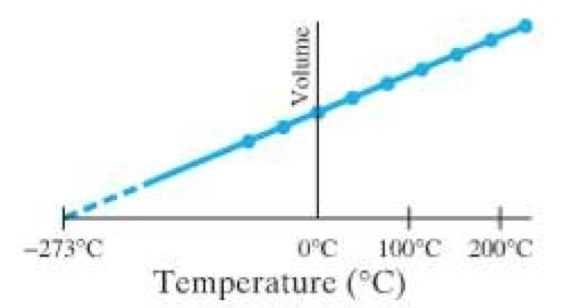
\includegraphics[scale=0.5]{VTgraph}
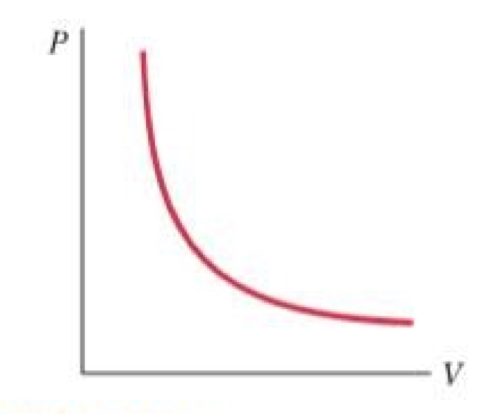
\includegraphics[scale=0.5]{PVgraph}
\caption{These graph always have x intercept at -273 degrees (0K), but more often the graph stops at liquefaction point (dotted) $\because$ it is impossible to have negative volume}
\end{figure}
\vspace{-20pt}
\section{Ideal Gas Law}
\begin{itemize}
\item By combining the three laws in the previous section, we have the general relation PV $\alpha$ T
\item Consider also how the amount of gas present affects system 
\item think of a blowing a balloon, V $\alpha $ n where n is the number of moles of gas \footnote{recall that number of moles can be found by $\frac{\text{mass (g)}}{\text{molar mass (g\/mol)}}$}
\item we now have PV $\alpha $ nT
\item To convert to an equality, we must introduce a constant of proportionality\footnote{remember to use K for ideal gas law calculation and absolute pressure} \\ R= gas constant =8.314 $\frac{J}{mol\cdot K}$
\item \textbf{STP }: T=273 K  P=1.00 atm=1.013$\times 10^{5} N/m^2$=101.3kPa
\item using the ideal gas law, it is easy to see that STP volume for 1 mole of \textbf{any gas} is 22.4 $m^3$ or Liters 
\end{itemize}
\section{Ideal Gas Law in Terms of Molecules: Avogadro's Number}
\begin{itemize}
\item Avogadro's hypothesis: equal volumes of gas at same P and T contain equal number of molecules
\item R is a constant for any gas $\because$ hypothesis and ideal gas law 
\item There are $N_A=6.02 \times 10^{23} \frac{\text{molecules}}{\text{mol}}$ number of molecules in one mole of any pure substance
\item We can figure this relation by dimensional analysis:
$$N=\text{ number of molecules} = [\frac{ molecules}{mol} \cdot mol] = n \cdot N_A$$
\item Rewriting Ideal Gas Law in terms of Boltzman constant:
\begin{align*}
k=&\text{Boltzman Constant}= \frac{R}{N_A}=\footnote{R can also be written as 8.314 $\frac{J}{mol \cdot K}$}
\frac{8.31\frac{kg \cdot m^2}{s^2 \cdot mol \cdot K}}{6.02 \times 10^{23}\frac{\text{molecules}}{\text{mol}}}=1.38 \times10^{-23} \frac{J}{K}
\\ &PV=nRT=\frac{N}{N_A} R T=NkT
\end{align*}
\end{itemize}
\section{Ideal Gas Temperature Scale -- a Standard}
\begin{itemize}
\item \textbf{ideal gas temperature scale}: universally-defined standard temperature measured by constant-volume gas thermometer \footnote{works on the principle of P$\alpha$ T @ constant V}
\item Like the Celsius and Fahrenheit scale, we need to specify two fixed points in order to set the scale.
\item So we choose P=0 at T=0K and the triple point of water.
\item Triple point of water is 4.58 torr (610.62 pascals)and 0.01$\,^{\circ}{\rm C} $; where water in solid ,liquid, and gas states can coexist in equilibrium
\item \textbf{Definition of the ideal gas temperature scale}:\\For an ideal gas in a constant-volume gas thermometer, we measure the absolute (Kelvin) temperature as:
$$T= (273.16 K)\lim_{P_{tp} \rightarrow 0}\frac {P}{P_{tp}} \quad \text{where $P_{tp}$ is the pressure of the gas at triple point}$$
\item Define triple point as 273.16K (when P=$P_{tp}$)
\item We use the limit $\because$ the temperature function is only an approximation (changes with the type of gas used in the thermometer). From graph, we can see that values for $P_{tp}>$0 varies and $P_{tp}$=0 for any type of gas. Therefore we take the limit of$ P_{tp} \rightarrow$0
\item Using this equation ($\because \lim$), the temperature is independent of the gas used. But make sure you use the gas with the right properties for measurement. \footnote{For example, you can not measure the absolute temperature under 1K with He,$\because$ Helium liquefies at 1K, lowest condensation point of all gases.}
\end{itemize}

$\quad \quad \quad  \quad \quad \quad \quad \quad \quad \quad \quad \quad \quad \quad \quad \quad \quad \quad \quad \quad \quad \quad \quad \quad \quad \quad \quad \quad \quad \quad \quad \textbf{Last Update:\today}$
\end{document}